% !TeX root = these.tex
\newpage
\chapter*{Annexes}

\setcounter{page}{1}
\pagenumbering{roman}
%\pagenumbering{Roman}
%\pagenumbering{Arabic}



\section{Formats de sérialisation RDF}
\label{annexe/serialisation}

% Pour les citer, voir Annexe \ref{annexe/serialisation}
% Important : compiler 2x

%\begin{figure}[!h]
%    \center
%   	\includegraphics[scale=0.75]{figureX.png}
%\end{figure}



\newpage


\section{Exemple de code}
\label{annexe/espace_nom}

\begin{figure}[!h]
\begin{lstlisting}[frame=single]
 from constraint import *
 problem = Problem()
 problem.addVariable("a", [1,2,3])
 problem.addVariable("b", [4,5,6])
 problem.getSolutions()
[{'a': 3, 'b': 6}, {'a': 3, 'b': 5}, {'a': 3, 'b': 4},
 {'a': 2, 'b': 6}, {'a': 2, 'b': 5}, {'a': 2, 'b': 4},
 {'a': 1, 'b': 6}, {'a': 1, 'b': 5}, {'a': 1, 'b': 4}]

 problem.addConstraint(lambda a, b: a*2 == b,
                          ("a", "b"))
 problem.getSolutions()
[{'a': 3, 'b': 6}, {'a': 2, 'b': 4}]

 problem = Problem()
 problem.addVariables(["a", "b"], [1, 2, 3])
 problem.addConstraint(AllDifferentConstraint())
 problem.getSolutions()
[{'a': 3, 'b': 2}, {'a': 3, 'b': 1}, {'a': 2, 'b': 3},
 {'a': 2, 'b': 1}, {'a': 1, 'b': 2}, {'a': 1, 'b': 3}]
\end{lstlisting}
\caption{Code python}
\end{figure}

\newpage


\section{Page de connexion et d'inscription}
\label{annexe/espace_nom}

\begin{figure}[!h]
	\begin{center}
		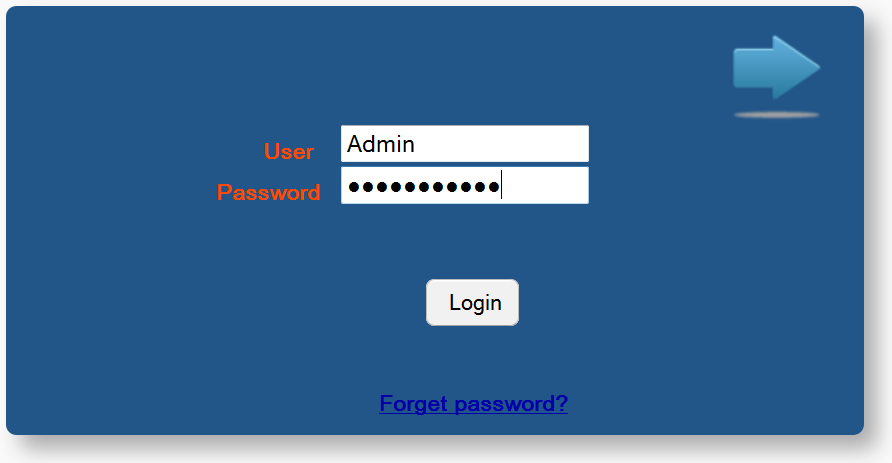
\includegraphics[width=16cm,height=8cm]{login.png}	
		\caption{page de connexion}
	\end{center}
\end{figure}

\begin{figure}[!h]
	\begin{center}
		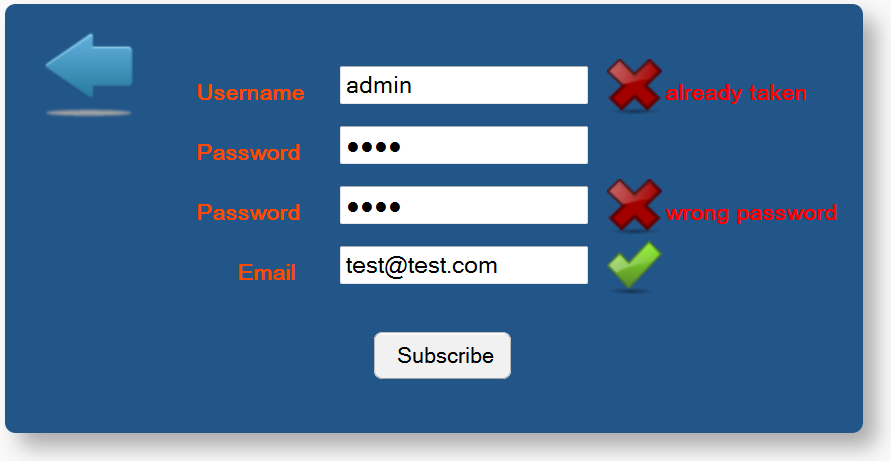
\includegraphics[width=16cm,height=8cm]{subscribe.png}
		\caption{page d'inscription}
	\end{center}
\end{figure}

\newpage

\section{Page des projets}
\label{annexe/espace_nom}

\begin{figure}[!h]
	\begin{center}
		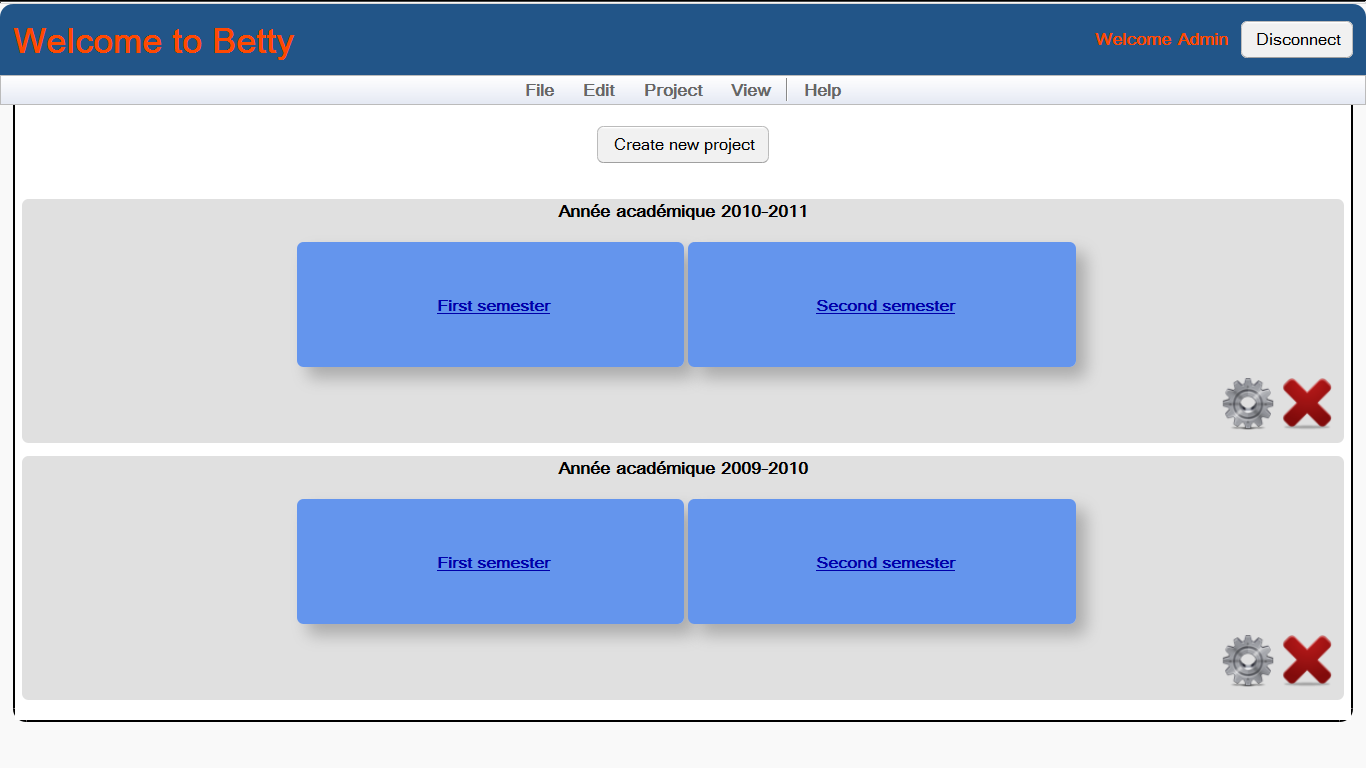
\includegraphics[width=19cm,height=12cm,angle=90]{ProjectPage.png}
		\caption{page des projets}
	\end{center}
\end{figure}\newpage

\newpage

\section{Page principale I}
\label{annexe/espace_nom}

\begin{figure}[!h]
	\begin{center}
		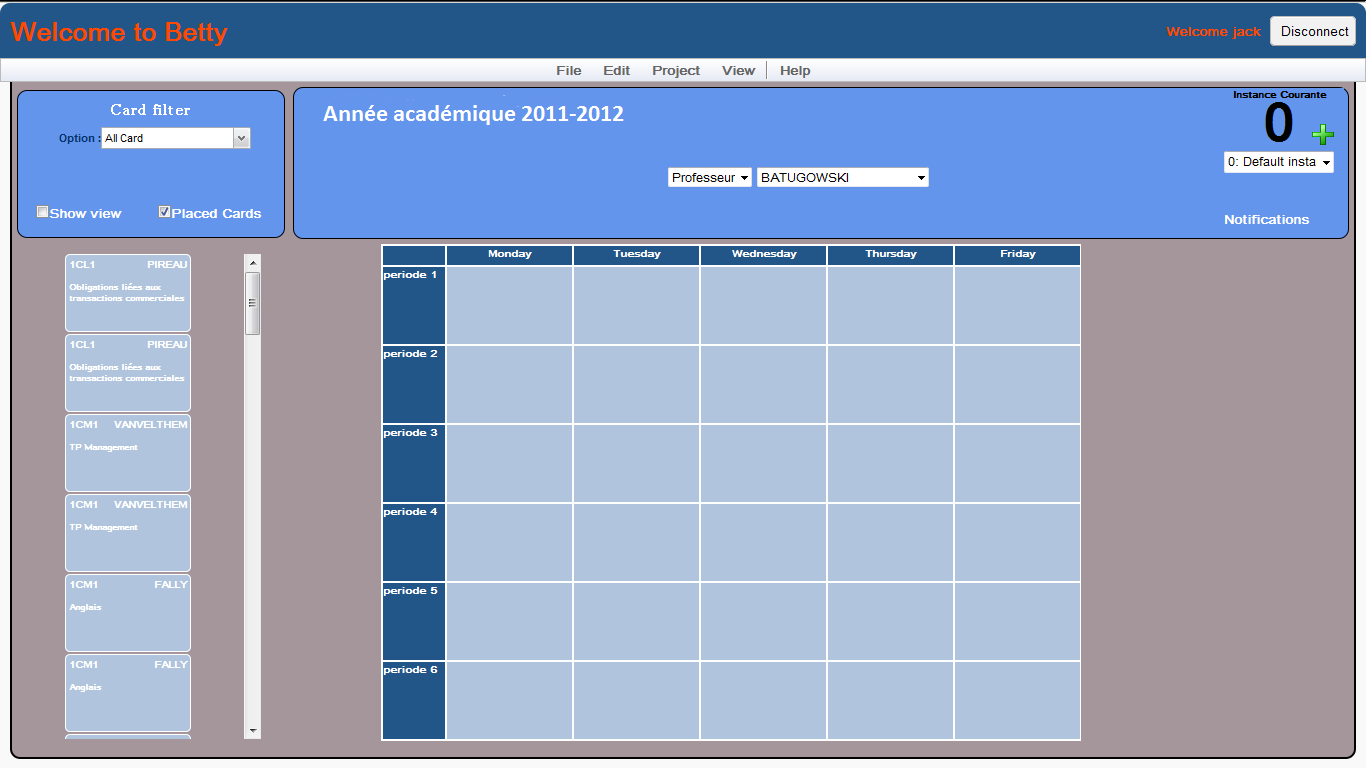
\includegraphics[width=19cm,height=12cm,angle=90]{MainPageClean.png}
		\caption{page principale vide}
	\end{center}
\end{figure}

\newpage

\section{Page principale II}
\label{annexe/espace_nom}

\begin{figure}[!h]
	\begin{center}
		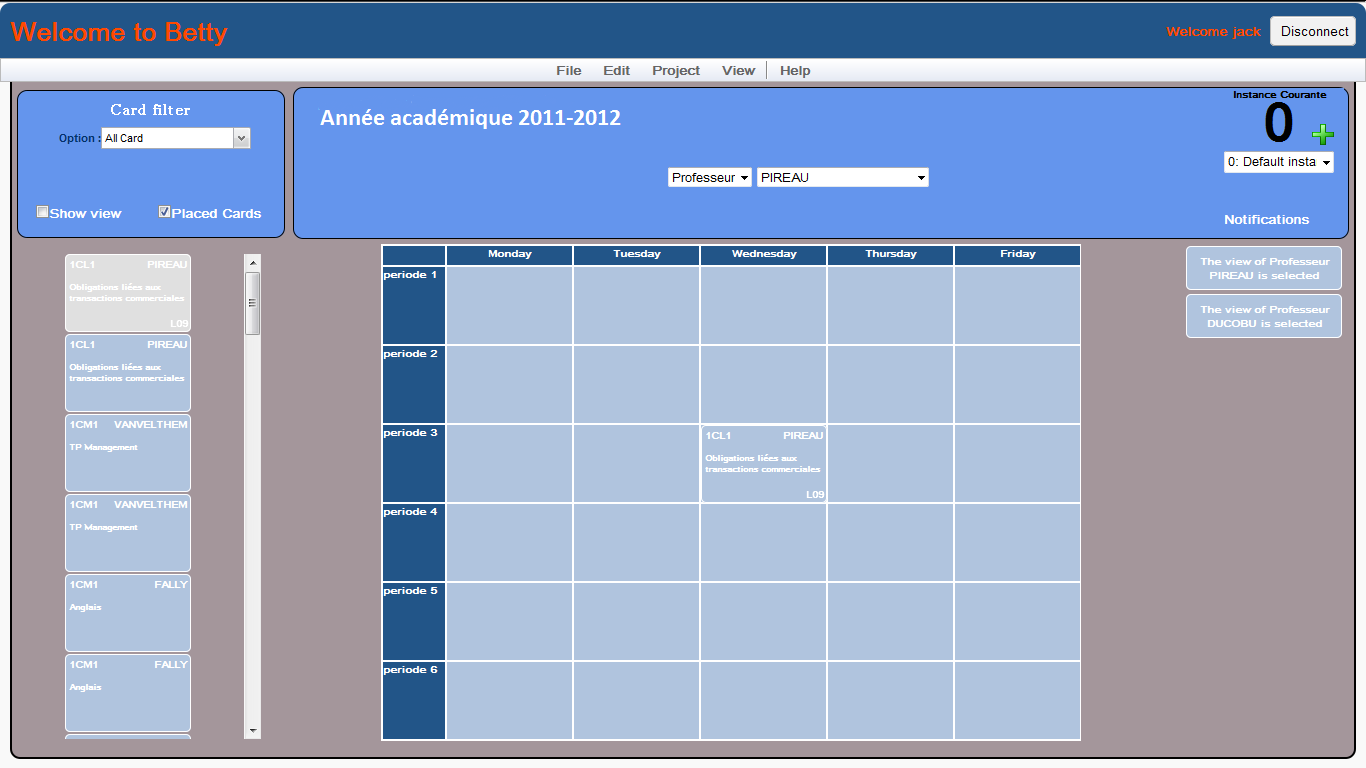
\includegraphics[width=19cm,height=12cm,angle=90]{MainPagePlacedCard.png}
		\caption{page principale carton placé}
	\end{center}
\end{figure}

\newpage

\section{Page principale III}
\label{annexe/espace_nom}

\begin{figure}[!h]
	\begin{center}
		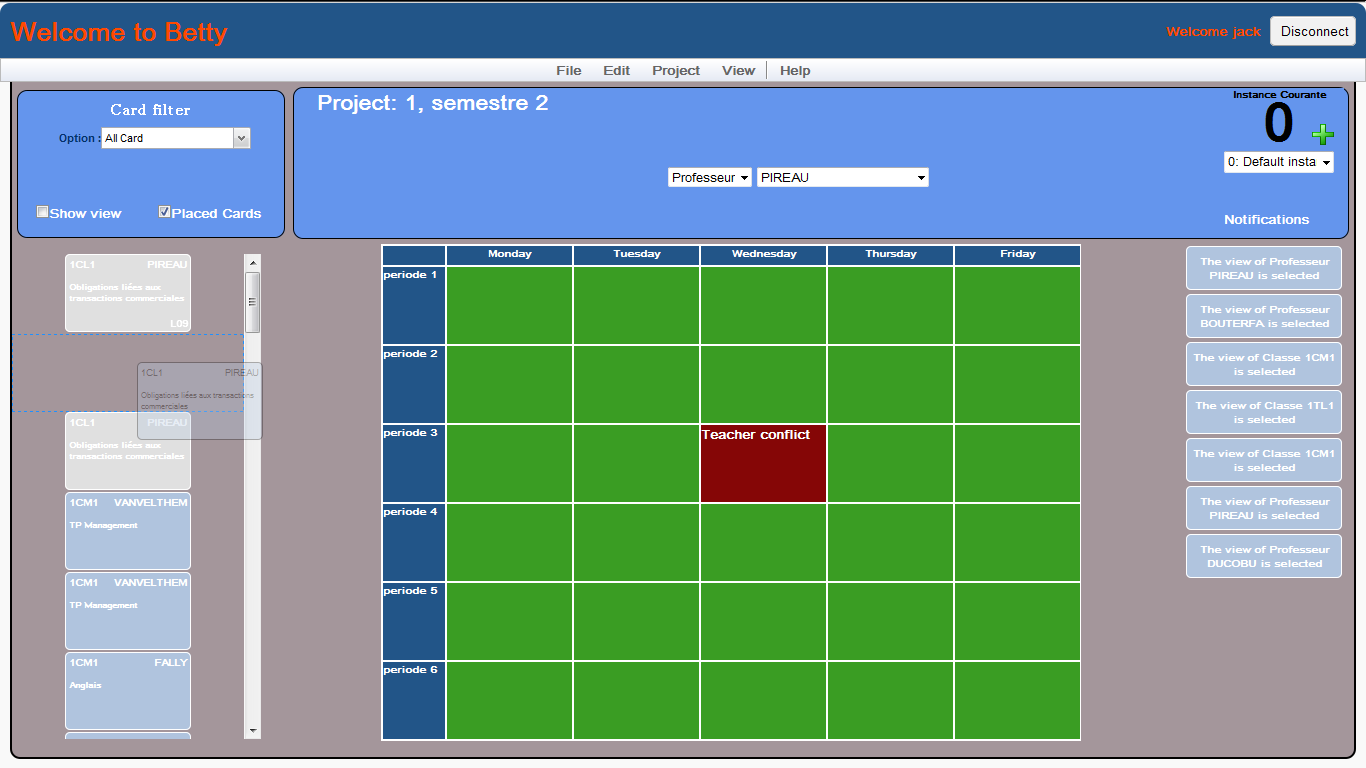
\includegraphics[width=19cm,height=12cm,angle=90]{MainPageColorTab.png}
		\caption{page principale solveur client}
	\end{center}
\end{figure}

\newpage

\section{Card filter}
\label{annexe/espace_nom}

\begin{figure}[!h]
	\begin{center}
		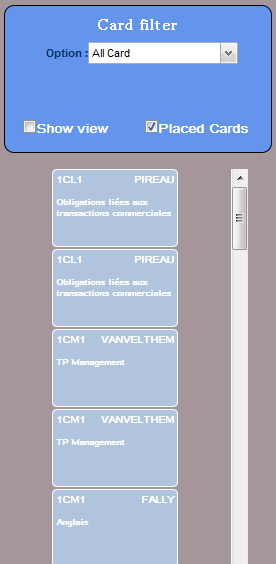
\includegraphics[width=6cm,height=12cm]{CardFilterAllCard.png}
		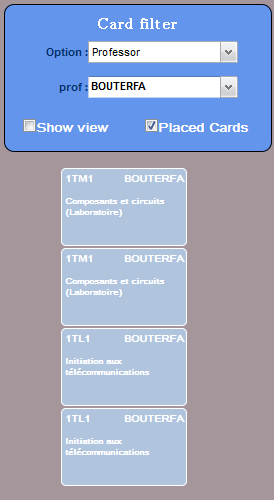
\includegraphics[width=6cm,height=10cm]{CardFilterBouterfa.png}
		\caption{présentation des cartons (non) filtrés}		
		\includegraphics[width=6cm,height=8cm]{CardFilterChoice.png}
		\caption{filtre avec multi-sélection}
	\end{center}
\end{figure}
